\chapter{{\tt Interest Point} Module}\label{ch:interestpoint-module}

[{\em Note: Parts of this documentation may no longer applicable... }]
$$
$$
Interest points are unique point identifiers with in an image. There
are usually many of them in an image and what defines them changes
based on the algorithm used. For the most part though, interest points
are defined at places where a corner exists, where at least 2 edges
come together.

Interest points are helpful in locating the same feature in multiple
images. There are 3 major parts to using interest points. First, all
images are processed with some interest point / corner detection and
all points are recorded. Secondly, all of the points found from the
first step now have a unique identifier built for them that properly
describes the feature and it texture surroundings. Lastly, captured
interest points are compared across images. Features on separate
images that have identifiers that seem approximately equal are then
connected into a match file.

Uses for interest points are general corner detection, object
recognition, and image alignment. The last one, image alignment, is a
common use used within Vision Workbench. Using fitting functors that
will be described later, transform matrices can be solved for to
describe the relationship between images and later merge them (see
{\tt <vw/Image/TransformView.h>}). Also as a side note, interest points
can be used for measurements for a bundle adjustment that would solve
for the original placement of the cameras (see
{\tt <vw/Camera/BundleAdjust.h>}).

The interest point module includes a complete set of classes and
functions for each step of interest point detection. They can be
imported into your code by including {\tt <vw/InterestPoint.h>}. The
built-in classes {\tt ScaledInterestPointDetector} and
{\tt SimpleInterestPointDetector} (defined in {\tt
  <vw/InterestPoint/Detector.h>}) provide out-of-the-box support for
detecting interest points, with or without scale space methods.

The interest point module is designed to be as flexible as possible in
that it decouples each step in the process of interest point
detection. Different interest measures and thresholding methods,
built-in or user-defined, can be used with the 
{\tt InterestPointDetector} classes. {\tt ScaledInterestPointDetector}
and {\tt SimpleInterestPointDetector} can both easily be subclassed to
further customize their operation, for example by implementing an
alternative method for finding peaks in the interest image.

The interest point module also provides tools for generating descriptors
to compactly describe the properties of an interest point.

\section{Scale Space Methods}
When detecting interest points, we want them to be invariant to changes in
view perspective. The scale space is a standard tool for making a
detection algorithm scale invariant \cite{lindeberg98}.

The interest point module provides support for scale space detection methods
based on the {\tt ImageOctave} class. An octave is a subset of the scale space.
It is a set of images (scales) formed by convolving the source image
with Gaussian kernels having progressively larger
standard deviations; the sigma used for the last scale in the octave is
twice that used for the first scale. Given a source image and a number of
scales per octave, {\tt ImageOctave} will construct the first octave of the
scale space of the source image. Successive octaves can be constructed
with the \verb#build_next()# method.

\begin{verbatim}
  ImageView<double> source;
  int scales_per_octave;
  ImageOctave octave(source, scales_per_octave);
  // Process first octave...
  // Then build the second octave
  octave.build_next();
\end{verbatim}

Building the next octave is a destructive operation, as the previously
computed octave data is not saved. If you need to retain all of the
scaled images generated, e.g. for use in generating descriptors,
{\tt ImageOctaveHistory} can be used to store this data.

\section{Measuring Interest}
The interest point module includes both classes and free functions
for computing interest images from source images using the
standard Harris \cite{harris88} and LoG (Laplacian of Gaussian)
interest measures. They can be imported by including the file
{\tt vw/InterestPoint/Interest.h}.

The HarrisInterest and LoGInterest classes are intended for use in
conjunction with the InterestPointDetector classes (next
section). Creating your own interest measure classes for use with the
Detector classes is straightforward.  Subclass the \verb#InterestBase#
abstract base type. In the constructor, set
\verb#InterestBase<T>::type# to \verb#IP_MIN#, \verb#IP_MAX# or
\verb#IP_MINMAX#, depending on what type of peaks in the generated
interest image represent interest points. Then overload the abstract
virtual method \verb#compute_interest# with your implementation of the
interest measure.

\section{The Interest Point Detector Classes}
The InterestPointDetector classes in
{\tt <vw/InterestPoint/Detector.h>} form the heart of the interest
point module. They integrate the various components of the module
into an easy all-in-one interface for detecting interest points.

The InterestPointDetector class itself is an abstract base class.
Two implementations of its interface are supplied,
{\tt ScaledInterestPointDetector} and {\tt SimpleInterestPointDetector}.
The Scaled version uses scale space methods, while the Simple version
does not; otherwise they are identical. When constructing either
type of detector, you specify an interest measure class and a
thresholding class. Built-in thresholding classes are defined in
{\tt <vw/InterestPoint/Threshold.h>}.

\begin{verbatim}
  LoGInterest<float> log;
  InterestThreshold<float> thresholder(0.0001);
  ScaledInterestPointDetector<float> detector(&log, &thresholder);
  std::vector<InterestPoint> points = interest_points(src, &detector);
\end{verbatim}

\section{Flow of Data}
Although designed primarily for flexibility, the interest point
module takes care not to sacrifice efficiency by unnecessarily
recomputing internal images such as gradients. If you take
advantage of the module's flexibility by customizing its
framework (for example, by implementing a new interest measure
class), you will probably make use of {\tt ImageInterestData}, a
struct which holds a source image and several interesting
related images, such as gradients and interest.

\section{Generating Descriptors}
A descriptor of an interest point represents the local image region
around the point. It should be distinctive as well as invariant to
factors such as illumination and viewpoint. The interest module
contains basic functions and classes for generating descriptors
in {\tt <vw/InterestPoint/Descriptor.h>}.

Generating a descriptor for an interest point requires knowledge
of the point's source image. Different descriptor classes may
require different source data. The trivial {\tt PatchDescriptor}
uses only the source {\tt ImageView} as its source data.

\begin{verbatim}
  SimpleInterestPointDetector<float> detector(&harris, &thresholder);
  std::vector<InterestPoint> points = interest_points(source_image,
                                                      &detector);
  PatchDescriptor<float> pd;
  generate_descriptors(points, source_image, pd);
\end{verbatim}

Properly generating descriptors for interest points found with
{\tt ScaledInterestPointDetector} is more involved, as various
blurred versions of the source image may be required to provide
local image regions for interest points at different scales.

\begin{verbatim}
  ScaledInterestPointDetector<float> detector(&log, &thresholder);
  ImageOctaveHistory<ImageInterestData<float> > history;
  detector.record_history(&history);
  SIFT_Descriptor<float> sd;
  generate_descriptors(points, history, sd);
\end{verbatim}

\section{Matching}

Aliens have abducted this section. Are you man enough to save it? Huh,
Punk?

\section{RANSAC}

RANdom SAmple Consensus {\em (or RANSAC)} is a method for sifting through
messy data to remove outliers. RANSAC starts with the goal of fitting
some objective to a mass of data. In the case of interest points it is
usually fitting some transform matrix to represent to move of points
from one image's coordinate frame to another. The algorithm works by
randomly selecting a minimal number of matches and fitting an initial
transform to this small selected set. It then proceeds to to grow the
initial set of matches from with matches from the original pool whose
error stays within an inlier threshold. This process of randomly
selecting a minimal set, fitting, and growing is repeated many
times. The round that produced the most inliers is kept for a final
stage where a better fitting algorithm can be applied to the entire
final pool of matches. The transform solved on the last step is
considered best solution that correctly maps the inliers. This shotgun
method, though not efficient, gives the ability for coping with a
large percentage of outliers. {\em Yet, also be aware that it is entirely
possible that in a worst case scenario, RANSAC might fit itself to an
interesting bunch of outliers.}

Vision Workbench's implementation can be found in 
{\tt <vw/Math/RANSAC.h>}. {\tt RandomSampleConsensus} expects 3 inputs
during it's construction. It requires a fitting functor that describes
the type of transform matrix used for fitting. It also needs an error
metric functor. For the case of interest points, 
{\tt InterestPointErrorMetric()} should do the job. Finally, an integer
describing the inlier threshold is required that defines the greatest
error allowed during fitting. An example of construction is below.

\begin{verbatim}
  vw::math::RandomSampleConsensus<math::SimilarityFittingFunctor,
                     math::InterestPointErrorMetric > ransac(
                     vw::math::SimilarityFittingFunctor(),
                     vw::math::InterestPointErrorMetric(), inlier_threshold );
\end{verbatim}

{\tt RandomSampleConsensus} is operated via an overloaded {\tt operator()}. 
It expects a container of Vector3s. Interest Point
module provides a helpful tool for converting to {\tt Vector3} from a
{\tt std::vector} of InterestPoints called {\tt
  iplist\_to\_vectorlist}. Finally the overloaded {\tt operator()} returns
it's final transform matrix result that was used to select it's
inliers, this can be stored for later image transform operations if
desired. {\tt RandomSampleConsensus} does not return a new list of inliers,
instead it returns the index locations of the inliers. It is left up
to the user to repackage the interest points to have only inliers. An
example of operations is below.

\begin{verbatim}
  std::vector<Vector3> ransac_ip1 = iplist_to_vectorlist(matched_ip1);
  std::vector<Vector3> ransac_ip2 = iplist_to_vectorlist(matched_ip2);
  
  Matrix<double> H(ransac(ransac_ip1,ransac_ip2));
  std::vector<int> indices = ransac.inlier_indices(H,ransac_ip1,ransac_ip2);
\end{verbatim}

Lastly, below is a listing of fitting functors that are available in
{\tt <vw/Math/Geometry.h>}.

\begin{table}[h]\begin{centering}
\begin{tabular}{|c|l|} \hline
Functor & Description \\ \hline \hline
\verb#HomographyFittingFunctor()# & 8 DOF. Also known as Projective matrix. \\ \hline
\verb#AffineFittingFunctor()# & 6 DOF. Handles rotation, translation, scaling, and skewing. \\ \hline
\verb#SimilarityFittingFunctor()# & 4 DOF. Handles rotation, translation, and scaling. \\ \hline
\verb#TranslationRotationFittingFunctor()# & 3 DOF. Also known as Euclidean matrix. \\ \hline
\end{tabular}
\caption{Fitting functors defined in {\tt <vw/Math/Geometry.h>}.}
\label{tbl:fitting-functors}
\end{centering}\end{table}

\section{Pre-built Tools}

To further help the introduction to the use of interest points,
Vision Workbench supplies two utility programs for working with interest
points. {\tt Ipfind} and {\tt Ipmatch} can be found built in
Vision Workbench's build path and the source code is available in {\tt
  <vw/tools/> }.

\begin{figure}[h]
\begin{center}
  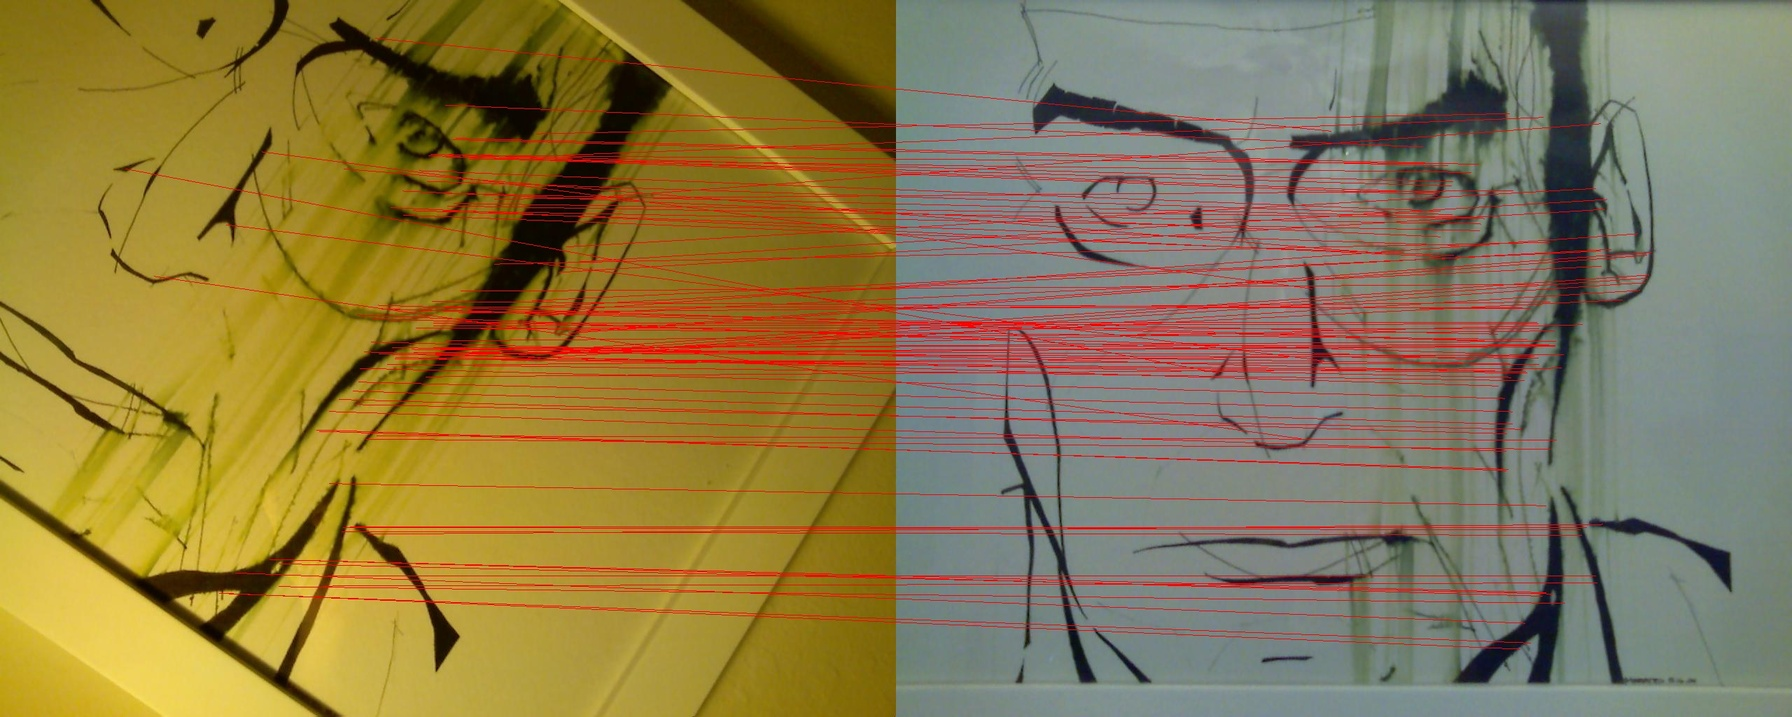
\includegraphics[width=6in]{images/ip_demo_match.jpg}
\end{center}
\caption{Example debug image from {\tt Ipmatch}.}
\label{fig:demo}
\end{figure}

The above is an example of a result that can be created with {\tt
  Ipfind} and {\tt Ipmatch}. Here are the commands used to create it.

\begin{verbatim}
  ipfind left.png right.png
  ipmatch left.png right.png -r homography -d
\end{verbatim}

\begin{thebibliography}{1}

\bibitem{harris88} Harris, Chris, and Mike Stephens, ``A Combined
  Corner and Edge Detector,'' Proc. 4th Alvey Vision Conf., Manchester,
  pp. 147-151, 1988.

\bibitem{lindeberg98} Lindeberg, Tony, ``Feature Detection with Automatic
  Scale Selection,''  Int. J. of Computer Vision, Vol. 30, number 2,
  1998.

\bibitem{lowe04} Lowe, David G., ``Distinctive Image Features from
  Scale-Invariant Keypoints,'' Int. J. of Computer Vision, 2004.

\end{thebibliography}
